
% v2-acmsmall-sample.tex, dated March 6 2012
% This is a sample file for ACM small trim journals
%
% Compilation using 'acmsmall.cls' - version 1.3 (March 2012), Aptara Inc.
% (c) 2010 Association for Computing Machinery (ACM)
%
% Questions/Suggestions/Feedback should be addressed to => "acmtexsupport@aptaracorp.com".
% Users can also go through the FAQs available on the journal's submission webpage.
%
% Steps to compile: latex, bibtex, latex latex
%
% For tracking purposes => this is v1.3 - March 2012
\documentclass[prodmode,acmtecs]{acmsmall} % Aptara syntax
\usepackage[spanish,polish]{babel}
\usepackage[T1]{fontenc}
\usepackage{fancyvrb}
\usepackage{graphicx,hyperref}
\newcommand\cutout[1]{}


\usepackage[table]{xcolor}
\usepackage[utf8]{inputenc}
\usepackage[parfill]{parskip}
\usepackage{tabulary}
\PassOptionsToPackage{hyphens}{url}
\usepackage{hyperref}    
\usepackage[capitalize]{cleveref}


% Metadata Information
% !!! TODO: SET THESE VALUES !!!
\acmVolume{0}
\acmNumber{0}
\acmArticle{CFP}
\acmYear{0}
\acmMonth{0}

\newcounter{colstart}
\setcounter{page}{4}

\RecustomVerbatimCommand{\VerbatimInput}{VerbatimInput}%
{
%fontsize=\footnotesize,
fontfamily=\rmdefault
}


\newcommand{\UnderscoreCommands}{%\do\verbatiminput%
\do\citeNP \do\citeA \do\citeANP \do\citeN \do\shortcite%
\do\shortciteNP \do\shortciteA \do\shortciteANP \do\shortciteN%
\do\citeyear \do\citeyearNP%
}

\usepackage[strings]{underscore}



% Document starts
\begin{document}


\setcounter{colstart}{\thepage}

\acmArticle{CFP}
\title{{\huge\sc SIGLOG Monthly 244}

 December 2023}
\author{DAVID PURSER\affil{University of Liverpool, UK}
\vspace*{-2.6cm}\begin{flushright}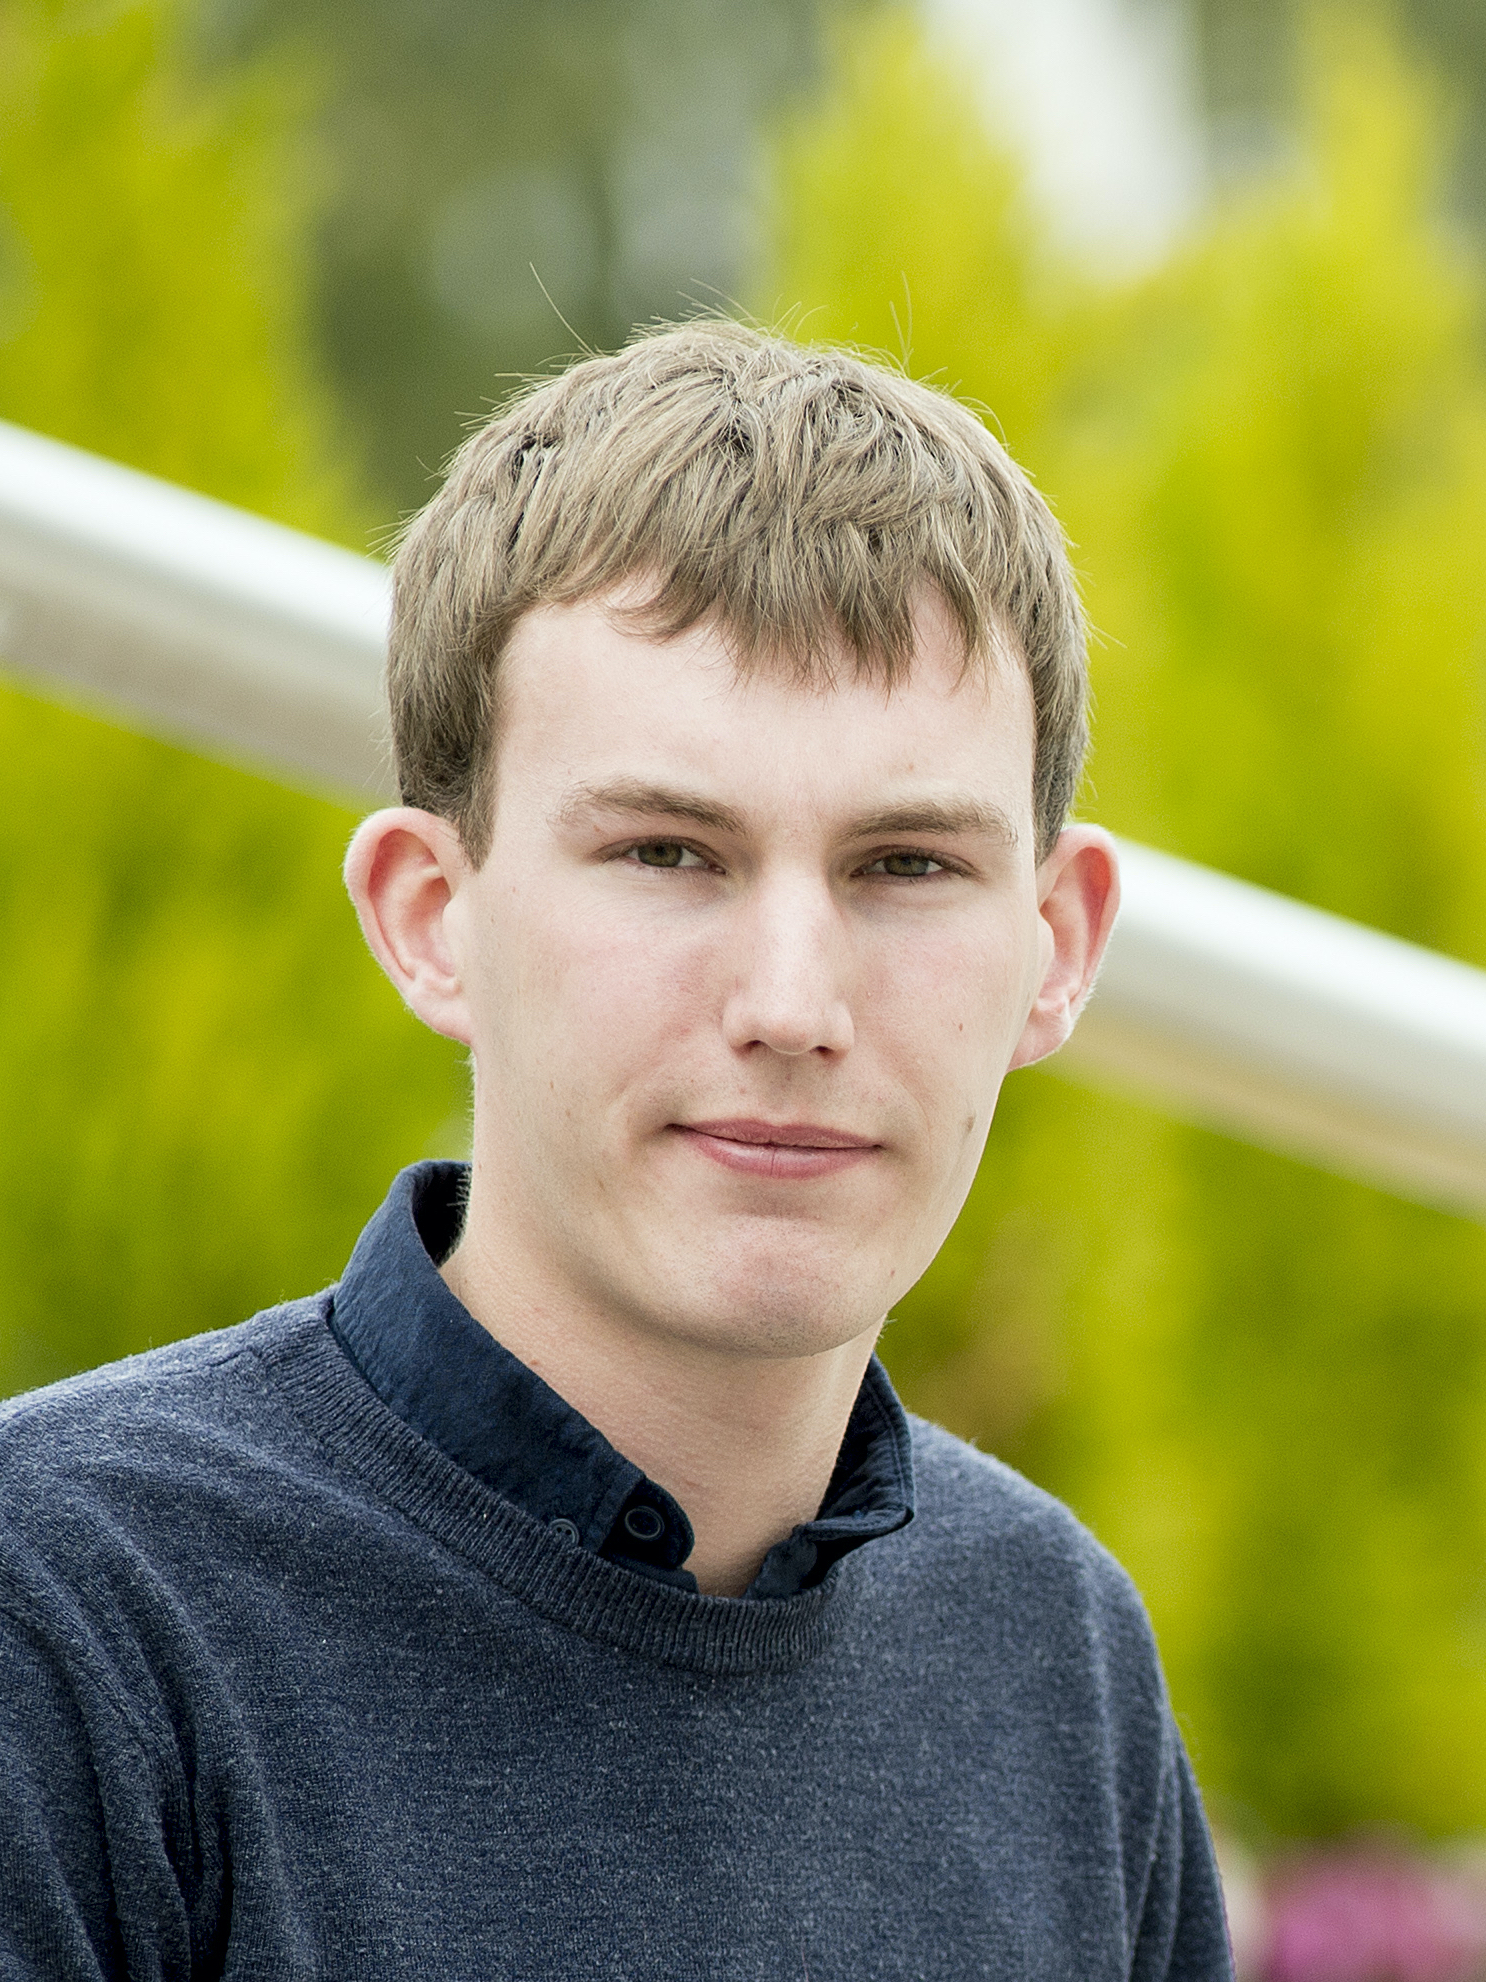
\includegraphics[width=30mm]{dp}\end{flushright}
}

\begin{abstract}
December 2023 edition of SIGLOG Monthly, featuring deadlines, calls and community announcements.
\end{abstract}


\maketitlee

\href{https://lics.siglog.org/newsletters/}{Past Issues}
 - 
\href{https://lics.siglog.org/newsletters/inst.html}{How to submit an announcement}
\section{Table of Content}\begin{itemize}\item DEADLINES (\cref{deadlines}) 
 
\item CALLS 
 
\begin{itemize}\item ICALP-LICS-FSCD (CALL FOR WORKSHOPS) (\cref{ICALPLICSFSCD})
\item ICGT 2024 (CALL FOR PAPERS) (\cref{ICGT2024})
\item Diagrams 2024 (CALL FOR PAPERS) (\cref{Diagrams2024})
\end{itemize} 
\item BOOK ANNOUNCEMENTS 
 
\begin{itemize}\item Computability and Complexity (\cref{ComputabilityandComplexity})
\end{itemize} 
\end{itemize}\section{Deadlines}\label{deadlines}\rowcolors{1}{white}{gray!25}\begin{tabulary}{\linewidth}{LL}FLOPS 2024:  & Dec 06, 2023 (Abstract), Dec 13, 2023 (Papers) \\
4 Positions at Oxford:  & Dec 13, 2023 (Deadline) \\
ICALP-LICS-FSCD:  & Dec 31, 2023 (Workshop proposals) \\
DEON2023:  & Jan 07, 2024 (Paper) \\
SPIN 2024:  & Jan 15, 2024 (Submissions) \\
CAV 2024:  & Jan 19, 2024 (Paper), Mar 01, 2024 (CAV Award Nomination deadline) \\
LICS 2024:  & Jan 21, 2024 (Titles and Short Abstracts), Jan 26, 2024 (Full Papers Due) \\
IJCAR 2024:  & Jan 29, 2024 (Abstract, extended), Feb 05, 2024 (Paper, extended), Dec 08, 2023 (Co-located event proposals, extended) \\
FSCD 2024:  & Feb 05, 2024 (Abstract), Feb 12, 2024 (Paper) \\
CiE 2024:  & Feb 10, 2024 (Article), May 15, 2024 (Informal presentations) \\
ICALP 2024:  & Feb 14, 2024 (Paper) \\
ICGT 2024:  & Feb 27, 2024 (Abstract), Mar 05, 2024 (Paper) \\
AiML 2024:  & Mar 08, 2024 (Abstract), Mar 15, 2024 (Full papers) \\
\end{tabulary}
\section{ICALP-LICS-FSCD}\label{ICALPLICSFSCD}	Tallinn, Estonia 8-13 July\\ 
CALL FOR WORKSHOPS 

\begin{itemize}\item  ICALP, LICS, and FSCD 2024 will be colocated in Tallinn, Estonia from 8th to 13th of July. 
 
  We invite proposals for workshops on topics of interest to the ICALP, LICS, and FSCD conferences. Note that workshops for ICALP track B and LICS will be joint this year. 
 
  Proposals must be limited to three pages and should be submitted to  icalp-lics-fscd-24-workshops@inria.fr .  
 
  Workshop proposals must include all the information listed at: \href{https://lics.siglog.org/lics24/cfw.php}{https://lics.siglog.org/lics24/cfw.php} 
 
  The organising and workshop committees of ICALP, LICS, and FSCD will determine the final list of accepted workshops based on topics and time/space availability. 
 
\item  IMPORTANT DATES 
 
\rowcolors{1}{white}{gray!25}\begin{tabulary}{\linewidth}{LL}Workshop proposals submission:  & Dec 31, 2023 \\
Notification of the accepted workshops:  & end of January, 2024 \\
Programme of the workshops ready:  & May 31, 2024 \\
ICALP track A Workshops dates:  & Jul 6-7, 2024 \\
ICALP track B / LICS Workshops dates:  & Jul 6-7, 2024 \\
FSCD Workshops dates:  & 8-9 and potentially 14 July, 2024 \\
ICALP Main conference:  & July 8-12, 2024 \\
LICS Main conference:  & July 8-11, 2024 \\
FSCD Main conference:  & July 10-13, 2024 \\
\end{tabulary}
 
\end{itemize}\section{ICGT 2024: 17th International Conference on Graph Transformation}\label{ICGT2024}  \href{https://conf.researchr.org/home/icgt-2024}{https://conf.researchr.org/home/icgt-2024}\\ 
  Part of STAF 2024, 8th-12th July in Twente, NL \href{https://conf.researchr.org/home/staf-2024}{https://conf.researchr.org/home/staf-2024}\\ 
CALL FOR PAPERS 

\begin{itemize}\item  AIMS AND SCOPE 
 
  The use of graphs and graph-like structures as a formalism for specification and modelling is widespread in all areas of computer science as well as in many fields of computational research and engineering. Relevant examples include software architectures, pointer structures, state space and control/data flow graphs, UML and other domain-specific models, network layouts, topologies of cyber-physical environments, quantum computing and molecular structures.  
 
  Often, these graphs undergo dynamic change, ranging from reconfiguration and evolution to various kinds of behaviour, all of which may be captured by rule-based graph manipulation. Thus, graphs and graph transformation form a fundamental universal modelling paradigm that serves as a means for formal reasoning and analysis, ranging from the verification of certain properties of interest to the discovery of fundamentally new insights. 
 
  The International Conference on Graph Transformation aims at fostering exchange and collaboration of researchers from different backgrounds working with graphs and graph transformation, either in contributing to their theoretical foundations or by applying established formalisms to classical or novel areas. The conference not only serves as a well-established scientific publication outlet, but also as a platform to boost inter- and intra-disciplinary research and provide leeway for new ideas. 
 
\item  IMPORTANT DATES 
 
  These dates are preliminary and may be slightly revised. 
 
\rowcolors{1}{white}{gray!25}\begin{tabulary}{\linewidth}{LL}Abstract submission:  & Feb 27, 2024 \\
Paper submission:  & Mar 05, 2024 \\
Notification:  & Apr 30, 2024 \\
Final version due:  & May 14, 2024 \\
Conference:  & within 8-12 Jul 2024 \\
\end{tabulary}
 
  All deadlines are by end-of-day, AoE 
 
\item  TOPICS 
 
  In order to foster a lively exchange of perspectives on the subject of the conference, the programme committee of ICGT 2024 encourages all kinds of contributions related to graphs and graph transformation, either from a theoretical point of view or a practical one. 
 
  Topics of interest include, but are not limited to the following subjects: General models of graph transformation (e.g. adhesive categories and hyperedge replacement systems); Analysis and verification of graph transformation systems; Structuring and modularisation of graph transformation; Hierarchical graphs and decomposition of graphs; Parallel, concurrent, and distributed graph transformation; Graph-theoretical properties of graph languages; Automata on graphs and parsing of graph languages; Logical aspects of graph transformation; Term graph and string diagram rewriting; Petri nets and other models of concurrency; Bigraphs and bigraphical reactive systems; Computational models based on graphs; Model checking, program analysis and verification, simulation and animation; Applications to computing paradigms (e.g. bio-inspired, quantum, ubiquitous, and visual); Graph databases and graph queries; Model-driven development and model transformation; Business process models and notations; Applications and case studies in software engineering (e.g. software architectures, refactoring, access control, and service-orientation); Syntax, semantics and implementation of programming languages, including domain-specific and visual languages; Graph transformation languages and tool support; Efficient algorithms (e.g. pattern matching, graph traversal, network analysis); Graph-based machine learning, including graph neural networks and models of rule inference; Graph transformation and artificial intelligence (e.g., AI for graph transformations, applying graph transformations in AI engineering and search-based software engineering)  
 
\item  SUBMISSION 
 
   For further information on paper types and submitting to ICGT see \href{https://conf.researchr.org/track/icgt-2024/icgt-2024-Research-Papers-1}{https://conf.researchr.org/track/icgt-2024/icgt-2024-Research-Papers-1} 
 
\end{itemize}\section{Diagrams 2024: 14th International Conference on the Theory and Application of Diagrams}\label{Diagrams2024}  September 27 – October 1, 2024\\ 
  University of Münster, Germany\\ 
  \href{https://diagrams-2024.diagrams-conference.org/}{https://diagrams-2024.diagrams-conference.org/}\\ 
CALL FOR PAPERS 

\begin{itemize}\item  The Diagrams conference provides a united forum for all researchers with an interest in the study of diagrams. The conference fosters multi-disciplinarity and allows researchers from areas such as computer science, mathematics, psychology, philosophy, history (of science, art, etc.), education research, and more to meet and share their perspectives on the theory and application of diagrams. 
 
\item  Further information: \href{https://diagrams-2024.diagrams-conference.org/calls/}{https://diagrams-2024.diagrams-conference.org/calls/} 
 
\end{itemize}\section{Computability and Complexity: written by Hubie Chen}\label{ComputabilityandComplexity}  published by The MIT Press (year 2023; 416 pages)\\ 
BOOK ANNOUNCEMENT 

\begin{itemize}\item  Publisher website for book: \href{https://mitpress.mit.edu/9780262048620/computability-and-complexity/}{https://mitpress.mit.edu/9780262048620/computability-and-complexity/} 
 
\item  Book excerpt:  An excerpt of this book, which includes the first chapter (of 4), is freely useable and freely distributable under a Creative Commons CC-BY-NC-ND license.  See the above website or use a direct link: \href{https://mitp-content-server.mit.edu/books/content/sectbyfn/books_pres_0/14340/CC_Book_selection.pdf}{https://mitp-content-server.mit.edu/books/content/sectbyfn/books\_pres\_0/14340/CC\_Book\_selection.pdf} . 
 
\item  Description: This initiation to the theory of computation covers the core notions, techniques, methods, and questions of this theory, before turning to several advanced topics.  This book combines intuitive and conceptual discussion—--backed by numerous diagrams and examples—--with a precise mathematical treatment that includes comprehensive and rigorous proofs.  Topics covered by this book include: 
 
\begin{itemize}\item  Automata theory – deterministic and nondeterministic finite automata, regular expressions, proving non-regularity via Myhill-Nerode theory, DFA minimization;
\item  Computability theory – deterministic and nondeterministic Turing machines, universal Turing machines, diagonalization and non-computable languages, reductions, Rice’s theorem;
\item  Complexity theory – time complexity classes (P, NP, and coNP), the P versus NP question, the theories of NP-completeness and of coNP-completeness, numerous completeness proofs, the space complexity class PSPACE, hierarchy theorems, fixed-parameter tractability, parameterized complexity.
\end{itemize} 
  Numerous exercises and notes expand upon the main presentation and cover topics such as Gödel incompleteness, counting complexity, logarithmic space complexity, and treewidth. 
 
\end{itemize}


\bigskip Links: \href{http://siglog.org/}{SIGLOG website}, \href{https://lics.siglog.org}{LICS website}, \href{https://lics.siglog.org/newsletters/}{SIGLOG Monthly}\end{document}